\section{Experimental Evaluation}
\label{eval}

\subsection{Datasets and evaluation protocol} \label{eval:protocol}
Our main dataset for experiments is the INRIA \emph{Holidays} dataset \cite{holidays}. This dataset consists of 1491 images divided in 500 groups of matching images. If the dataset of an experiment is not mentioned in what follows this means, by default, that it is performed on \emph{Holidays}.
We also use  the \emph{Oxford5k} dataset \cite{oxford}, which consists of 5062 images separated in 55 groups of matching images.

In both datasets, each group contains one query image, the other images in the group being the only correct answers to the query. 
For each query image, we calculate its similarity to all other images in the database and rank them, in decreasing order. 
The average precision of a group is derived from the ranking of the images of the group for the similarity with the corresponding query image. 
The final mean average precision (mAP) for a dataset is the mean of the average precision over all its groups.
As pool of negative images to build E-SVM adn SLEM representations, we use the Flickr100k collection \cite{oxford}, composed of $10^5$ images from Flickr. For a full rank decomposition, we use only a subset of it, containing between 6000 and 15000 images. 
As stated in section \ref{low-rank} and further discussed in section \ref{time-scale}, a full rank decomposition does not scale well for bigger number of negative samples. For low rank decomposition, we use all 100000 images.

At evaluation time, for a dataset that consists of $p$ images and $q$ query images, we calculate its $p\times q$ \emph{similarity matrix} $S$, where each of its $q$ columns is the matching scores of the query image with all the $p$ images.


\subsection{Which kernel to choose?}
We tested three different kernels --linear, Gaussian and polynomial-- each with a scalar parameter $\gamma$:
\begin{align}
    &k_{linear}(x,y) = x^Ty, \label{k:lin}\\
    &k_{gauss}(x,y) = \exp(-\gamma\|x-y \|^2), \label{k:rbf}\\
    &k_{poly}(x,y) = x^Ty+\gamma(x^Ty)^2. \label{k:poly}\\
    %&k_{spp}(x,y) = \dfrac{1}{2^L}\mathcal{I}(H^0_x, H^0_y) +\sum_{l=1}^L\dfrac{1}{2^{L-l+1}}\mathcal{I}(H^{l,\gamma}_x, H^{l,\gamma}_y). \label{k:spm}
\end{align}
\textbf{Linear SLEM} The linear kernel of Equation (\ref{k:lin}) is the first default choice and equivalent to the non-kernelized version of SLEM.
In the remaining of this paper, we reference to linear SLEM when we use the non-kernelized SLEM.
\textbf{Gaussian SLEM} The radial basis function kernel of Equation (\ref{k:rbf}) is a
well known reproducing kernel, used for classification with support vector machines.
\textbf{Polynomial SLEM} The polynomial kernel of Equation (\ref{k:poly}) is a reproducing kernel often used in natural language processing. 
%\textbf{SPM SLEM} The spatial pyramid matching kernel of $L+1$ levels in Equation \ref{k:spm} take as input a set of local descriptors and its location in pyramidal bins \cite{spk}. 


\subsection{Base visual features}
We test our feature encoder for three different base features $x\in\mathbb{R}^d$, one hand-crafted image representation and two learned from deep convolutional neural networks.


We revisit the VLAD feature presented in \cite{VLAD} as an example of a hand-crafted representation. First we extract a set $\mathcal{F}$ of local descriptors of the image $I$. We use the 128 dimension RootSIFT \cite{3things} descriptors, extracted densely. 
Then, we hard-assign each descriptor $f$ in $\mathcal{F}$ to the closest among $K$ pre-trained codewords $c_k$, $k\in\{1\cdots K\}$,
%one of $K$ set $\mathcal{C}_k$ of descriptors associated to codewords $\{c_k\}_{1\leq k\leq K}$, 
and map $f$ to a $\RR^{128K}$ vector 
\begin{equation}
\phi^{VL}_1(f) = \left[0 \cdots 0\quad \Phi_k^T\frac{(f-c_k)}{\|f-c_k\|} \quad 0 \cdots 0\right],
\end{equation}
where $\Phi_k$ is a $128\times 128$ PCA matrix learned on training features mapped to $k$-the codeword.
%associated to descriptors in $\mathcal{C}_k$. 
The final VLAD representation is the power-normalization and $l_2$ normalization of the sum-pooling of $\phi^{VL}_1$:
\begin{equation}
\phi^{VL}_2(I) \propto \mathrm{power}\big(\sum_{f\in \mathcal{F}}\phi^{VL}_1(f)\big),~\|\phi^{VL}_2(I)\|=1,
\end{equation}
with scalar power normalization $\mathrm{power}(v)=\mathrm{sign}(v)|v|^{0.5}$ applied component-wise.
In experiments, we use $K=64$ codewords learned on images from Flickr. Our VLAD representation has $d=8192$ dimensions.

Convolutional features obtained from very deep convolutional neural networks (CNNs) have been shown to work as good local descriptors for matching \cite{SimonZisser15}. The SPoC representation \cite{babenko15} is a weighted sum-pooling of the activations of the last convolutional layer of a 19-layer CNN. For a given input image $I$, the activations in this layer are organized over a $W\times H$ spatial grid and over $d$ channels. Each position $(w,h)\in \{1 \cdots W\}\times \{1\cdots H\}$ can thus be equipped with a descriptor $f_{h,w}(I)\in\RR^D$. 
%Indeed, if our last convolutional layer has $D$ neurons, and each neuron a $W\times H$ map of activations of this neurons to the image $I$, 
%each pair $(w,h)$ with $w$ in $\{1,2,..., W\}$ and $h$ in $\{1,2,...,H\}$ can be associated to a descriptor $f_{(h,w)}$ in $\RR^D$ of the responses of each neuron at coordinate $(w,h)$ of the maps. 
We then sum-pool these descriptors, weighted accordingly to their distance to the center of the image:
\begin{equation}
    \phi^{SPoC}(I) = \sum_{w=1}^W\sum_{h=1}^H \alpha_{w,h}f_{w,h}(I),
\end{equation}
where
\begin{equation}
    \alpha_{w,h} = \exp \left(-\dfrac{(w-W/2)^2+(h-H/2)^2}{2\sigma^2}\right).
\end{equation}
In our experiments, we follow the implementation details of \cite{babenko15}: We resize all images to $586\times 586$ pixels before feeding them to the network. The last convolutional layer has $d=512$ channels with activation maps of size $(W,H)=(37,37)$. We also set $\sigma=\frac{H}{3}$.

Finally, we also test a more convencional CNN feature, less deep and using two fully connected layers after the convolutional layers. 
Our final representation is a $4096$ non-negative feature. We based out implementation on CAFFE \ref{jia2014caffe}.


\subsection{Implementation details}
We cross validate $\gamma$ and $\lambda$ for Poly and Gaussian SLEM. to be completed


\subsection{Full rank results}

We test our method against the established ESVM and PCA. 
\cite{babenko15} improves the retrieval results of SPoC by applying a PCA compression followed by whitening. In our experiments, the compression worsen the results when compared with non-compressed.
Hence we compare the improvements of PCA plus whitening, without compression, with our method.
Linear SLEM performs similarly to ESVM despite being much more time efficient (see discussion in section \ref{time-scale}). 
Gaussian SLEM and Polynomial SLEM outperform all methods, for all datasets and all image representations. 
The results are presented in Table \ref{fullrank:results}.

\begin{table*}[t]
\begin{center}
\caption{Mean average precision results for INRIA Holidays and Oxford buildings datasets, expressed as percentages. In this table, we present our results for VLAD-64 \ref{VLAD}, sum-pooling of convolutional features (SPoC) \ref{babenko15} and fully connected (fc) CNN \ref{jia2014caffe}}
\begin{tabular}{|c|c|c|c|c|c|c|c|}
\hline
Dataset & \multicolumn{3}{|c|}{\textbf{Holidays}} & \multicolumn{3}{|c|}{\textbf{Oxford 5k}}\\
\hline
Method, features & VLAD-64  & SPoC CNN & FC CNN & VLAD-64 & SPoC CNN & FC CNN\\
\hline\hline
Baseline            & 72.7 & 73.1 & 68.2  & 46.3 & 54.4 & 40.6\\
%Whitening           & -    & -    & -    & -    & -\\
PCA+whitening       & 69.4 & 77.5 & 69.2 & 50.9  & 63.7 & 45 \\
E-SVM               & 78.3 & 79.9 & 71.8 & 57.5  & 62.1 & 44.6\\
Linear SLEM         & 78   & 78.3 & 72.1 & 57.5  & 64.1 & 45.5\\
Gaussian SLEM       & 78.1 & 81.4 & 72.9 & 59    & 64.9 & 46.1\\
Poly SLEM           & 78.1 &  82  & 72.9 & 59.3  & 64.8 & 46\\
\hline
\end{tabular}
\end{center}
\label{fullrank:results}
\end{table*}

\subsection{Time Scalability} \label{time-scale}
In this section we compare the time efficiency of our method and the E-SVM, as well as discuss which method to use accordingly with the number of positive and negative samples.

In Figure \ref{fullrank:results}, we see Linear SLEM efficiency does not change with $n$. 
Indeed, if $d$ is the dimension of the base representation, $A$ is a $d\times d$ matrix for Linear SLEM, whereas for a full rank kernel, $A$ is a $n\times n$. 
This explain the increasing running time for Gaussian and polynomial kernels: storage and solving a $n\times n$ system does not scale for large number of negative samples. 
But retrieval results in Figure \ref{fullrank:results} suggest we can benefit from larger sets of negative samples. Linear SLEM and ESVM scales well, but do not perform so well. 
\vspace{3 mm}
\begin{figure}
  \begin{tikzpicture}
    \begin{groupplot}
      [group style={%
        columns=2,
        rows=1,
        group name=plots,
        xlabels at=edge bottom,
        %y descriptions at=all,
        horizontal sep=5em,        
      },
      % ybar,
      % ymin=0,
      % ymax=27e3,
      enlarge x limits={abs=.5},
      width=0.5\textwidth,
      height=0.4\textwidth,
      % scaled y ticks=base 10:-3,
      % xticklabels from table={\first}{Criterion},
      % x tick label style={rotate=90,anchor=east},
      % xtick=data,
      ]

      \nextgroupplot[xlabel=Num. of negatives,
      ylabel=mAP]
      ]
      %% Poly SLEM
      \addplot[PolySLEM] coordinates {
        (500,  0.78852)
        (1500, 0.80397)
        (2500, 0.80648)
        (3500, 0.80905)
        (4500, 0.81192)
        (5500, 0.81502)
        (6500, 0.81659)
        (7500, 0.81712)
        (8500, 0.81599)
        (9500, 0.81432)
        (10500,0.81625)
        (11500,0.81796)
        (12500,0.81726)
        (13500,0.81993)
        (14500,0.82057)
      };
      %% Gaussian SLEM
      \addplot[GaussSLEM] coordinates {
        (500,  0.77757)
        (1500, 0.79756)
        (2500, 0.80338)
        (3500, 0.79909)
        (4500, 0.79950)
        (5500, 0.80257)
        (6500, 0.8016)
        (7500, 0.80362)
        (8500, 0.80377)
        (9500, 0.80501)
        (10500,0.80534)
        (11500,0.80909)
        (12500,0.80955)
        (13500,0.80813)
        (14500,0.81214)
      };
      %% ESVM
      \addplot[ESVM] coordinates {
        (500,  0.7684)
        (1500, 0.78434)
        (2500, 0.78836)
        (3500, 0.78927)
        (4500, 0.79292)
        (5500, 0.79523)
        (6500, 0.79491)
        (7500, 0.79557)
        (8500, 0.79915)
        (9500, 0.79819)
        (10500,0.79888)
        (11500,0.7985)
        (12500,0.79822)
        (13500,0.79930)
        (14500,0.79905)
      };
      %% Linear SLEM
      \addplot[LinSLEM] coordinates {
        (500,  0.77638)
        (1500, 0.7748)
        (2500, 0.77919)
        (3500, 0.77914)
        (4500, 0.7748)
        (5500, 0.77578)
        (6500, 0.77902)
        (7500, 0.78338)
        (8500, 0.78043)
        (9500, 0.78026)
        (10500,0.77803)
        (11500,0.77767)
        (12500,0.77818)
        (13500,0.78148)
        (14500,0.78254)
      };

      \nextgroupplot[
      ymode=log,
      xlabel=Num. of negatives,
      ylabel=Time per image (s),
      legend to name=grouplegend,
      legend style={legend columns=-1},
      % legend style={at={(0.465,-0.45)},
      % anchor=north,legend columns=-1},
      ]%
      %% Poly SLEM
      \addplot[PolySLEM] coordinates {
        (500,  0.0001)
        (1500, 0.0007)
        (2500, 0.0023)
        (3500, 0.0046)
        (4500, 0.0088)
        (5500, 0.0146)
        (6500, 0.0213)
        (7500, 0.0289)
        (8500, 0.0395)
        (9500, 0.0542)
        (10500,0.0703)
        (11500,0.0903)
        (12500,0.1103)
        (13500,0.1434)
        (14500,0.1745)
      };
      \addlegendentry{Poly SLEM}
      %% Gaussian SLEM
      \addplot[GaussSLEM] coordinates {
        (500,  0.0003)
        (1500, 0.0008)
        (2500, 0.0021)
        (3500, 0.0044)
        (4500, 0.0072)
        (5500, 0.0119)
        (6500, 0.0172)
        (7500, 0.026)
        (8500, 0.0344)
        (9500, 0.0465)
        (10500,0.0617)
        (11500,0.0814)
        (12500,0.1248)
        (13500,0.1301)
        (14500,0.161)
      };
      \addlegendentry{Gaussian SLEM}
      %% ESVM
      \addplot[ESVM] coordinates {
        (500,  0.014)
        (1500, 0.015)
        (2500, 0.016)
        (3500, 0.017)
        (4500, 0.018)
        (5500, 0.019)
        (6500, 0.02)
        (7500, 0.021)
        (8500, 0.022)
        (9500, 0.023)
        (10500,0.024)
        (11500,0.025)
        (12500,0.026)
        (13500,0.027)
        (14500,0.028)
      };
      \addlegendentry{ESVM}
      %% Linear SLEM
      \addplot[LinSLEM] coordinates {
        (500,  0.0000565)
        (1500, 0.0000575)
        (2500, 0.0000467)
        (3500, 0.0000679)
        (4500, 0.0000683)
        (5500, 0.0000612)
        (6500, 0.0000608)
        (7500, 0.0000708)
        (8500, 0.0000743)
        (9500, 0.0000996)
        (10500, 0.0000993)
        (11500,0.0001073)
        (12500,0.0001027)
        (13500,0.000075)
        (14500,0.0001141)
      };
      \addlegendentry{Linear SLEM}
      


    \end{groupplot}

    \node at (plots c1r1.north east) [anchor=south, xshift=2.5em] {\ref{grouplegend}};
    %\draw (plots c2r1.north west) circle (3pt) node {North west};

  \end{tikzpicture}
  \caption{Results for INRIA Holidays, using SPoC features and different methods of SLEM (see legend).}
  \label{fullrank:results}
\end{figure}


% \begin{figure}
%   \begin{tikzpicture}
%     \begin{groupplot}
%       [group style={%
%         columns=3,
%         group name=plots,
%         xlabels at=edge bottom,
%         y descriptions at=edge left,
%       },
%       ybar,
%       ymin=0,
%       ymax=27e3,
%       enlarge x limits={abs=.5},
%       width=0.35\textwidth,
%       height=0.6\textwidth,
%       scaled y ticks=base 10:-3,
%       xticklabels from table={\first}{Criterion},
%       x tick label style={rotate=90,anchor=east},
%       xtick=data,
%       ]

%       \nextgroupplot[xlabel=item1,legend to name=grouplegend,ylabel=y-label]
%       \pgfplotstableforeachcolumn\first\as\col{%
%         \ifnum\pgfplotstablecol=0
%         \else
%         \edef\tmp{%
%           \noexpand\addplot table [x expr=\noexpand\coordindex,y=\col] {\noexpand\first};
%           \noexpand\addlegendentry {\col}%
%         }%
%         \tmp
%         \fi
%       }

%       \nextgroupplot[xlabel=item2]
%       \pgfplotstableforeachcolumn\second\as\col{%
%         \ifnum\pgfplotstablecol=0 
%         \else
%         \edef\tmp{%
%           \noexpand\addplot table [x expr=\noexpand\coordindex,y=\col] {\noexpand\second};
%         }%
%         \tmp
%         \fi
%       }

%       \nextgroupplot[xlabel=item3]
%       \pgfplotstableforeachcolumn\third\as\col{%
%         \ifnum\pgfplotstablecol=0 
%         \else
%         \edef\tmp{%
%           \noexpand\addplot table [x expr=\noexpand\coordindex,y=\col] {\noexpand\third};
%         }%
%         \tmp
%         \fi
%       }
%     \end{groupplot}

%     \node at (plots c2r1.north) [anchor=south, yshift=.6cm] {\ref{grouplegend}};
%   \end{tikzpicture}
% \end{figure}


% \def\sideboxwidth{0.48\textwidth}
% \def\centerboxwidth{0.02\textwidth}
% \begin{figure}[!h]
%   \begin{minipage}{\sideboxwidth}
%     \begin{center}
%       \begin{tikzpicture}
% 	\begin{axis}[
%           xlabel=Num. of negatives,
%           ylabel=mAP]
%           %% Poly SLEM
%           \addplot[PolySLEM] coordinates {
%             (500,  0.78852)
%             (1500, 0.80397)
%             (2500, 0.80648)
%             (3500, 0.80905)
%             (4500, 0.81192)
%             (5500, 0.81502)
%             (6500, 0.81659)
%             (7500, 0.81712)
%             (8500, 0.81599)
%             (9500, 0.81432)
%             (10500,0.81625)
%             (11500,0.81796)
%             (12500,0.81726)
%             (13500,0.81993)
%             (14500,0.82057)
%           };
%           %% Gaussian SLEM
%           \addplot[GaussSLEM] coordinates {
%             (500,  0.77757)
%             (1500, 0.79756)
%             (2500, 0.80338)
%             (3500, 0.79909)
%             (4500, 0.79950)
%             (5500, 0.80257)
%             (6500, 0.8016)
%             (7500, 0.80362)
%             (8500, 0.80377)
%             (9500, 0.80501)
%             (10500,0.80534)
%             (11500,0.80909)
%             (12500,0.80955)
%             (13500,0.80813)
%             (14500,0.81214)
%           };
%           %% ESVM
%           \addplot[ESVM] coordinates {
%             (500,  0.7684)
%             (1500, 0.78434)
%             (2500, 0.78836)
%             (3500, 0.78927)
%             (4500, 0.79292)
%             (5500, 0.79523)
%             (6500, 0.79491)
%             (7500, 0.79557)
%             (8500, 0.79915)
%             (9500, 0.79819)
%             (10500,0.79888)
%             (11500,0.7985)
%             (12500,0.79822)
%             (13500,0.79930)
%             (14500,0.79905)
%           };
%           %% Linear SLEM
%           \addplot[LinSLEM] coordinates {
%             (500,  0.77638)
%             (1500, 0.7748)
%             (2500, 0.77919)
%             (3500, 0.77914)
%             (4500, 0.7748)
%             (5500, 0.77578)
%             (6500, 0.77902)
%             (7500, 0.78338)
%             (8500, 0.78043)
%             (9500, 0.78026)
%             (10500,0.77803)
%             (11500,0.77767)
%             (12500,0.77818)
%             (13500,0.78148)
%             (14500,0.78254)
%           };
% 	\end{axis}
%       \end{tikzpicture}
%     \end{center}
%   \end{minipage}%
%   \begin{minipage}{\centerboxwidth}~\end{minipage}%
%   \begin{minipage}{\sideboxwidth}
%     \begin{center}
%       \begin{tikzpicture}
% 	\begin{semilogyaxis}[
%           xlabel=Num. of negatives,
%           ylabel=Time per image (s),
%           legend style={at={(0.465,-0.45)},
%             anchor=north,legend columns=-1},
%           ]%legend pos=outer south]
%           %% Poly SLEM
%           \addplot[PolySLEM] coordinates {
%             (500,  0.0001)
%             (1500, 0.0007)
%             (2500, 0.0023)
%             (3500, 0.0046)
%             (4500, 0.0088)
%             (5500, 0.0146)
%             (6500, 0.0213)
%             (7500, 0.0289)
%             (8500, 0.0395)
%             (9500, 0.0542)
%             (10500,0.0703)
%             (11500,0.0903)
%             (12500,0.1103)
%             (13500,0.1434)
%             (14500,0.1745)
%           };
%           \addlegendentry{Poly SLEM}
%           %% Gaussian SLEM
%           \addplot[GaussSLEM] coordinates {
%             (500,  0.0003)
%             (1500, 0.0008)
%             (2500, 0.0021)
%             (3500, 0.0044)
%             (4500, 0.0072)
%             (5500, 0.0119)
%             (6500, 0.0172)
%             (7500, 0.026)
%             (8500, 0.0344)
%             (9500, 0.0465)
%             (10500,0.0617)
%             (11500,0.0814)
%             (12500,0.1248)
%             (13500,0.1301)
%             (14500,0.161)
%           };
%           \addlegendentry{Gaussian SLEM}
%           %% ESVM
%           \addplot[ESVM] coordinates {
%             (500,  0.014)
%             (1500, 0.015)
%             (2500, 0.016)
%             (3500, 0.017)
%             (4500, 0.018)
%             (5500, 0.019)
%             (6500, 0.02)
%             (7500, 0.021)
%             (8500, 0.022)
%             (9500, 0.023)
%             (10500,0.024)
%             (11500,0.025)
%             (12500,0.026)
%             (13500,0.027)
%             (14500,0.028)
%           };
%           \addlegendentry{ESVM}
%           %% Linear SLEM
%           \addplot[LinSLEM] coordinates {
%             (500,  0.0000565)
%             (1500, 0.0000575)
%             (2500, 0.0000467)
%             (3500, 0.0000679)
%             (4500, 0.0000683)
%             (5500, 0.0000612)
%             (6500, 0.0000608)
%             (7500, 0.0000708)
%             (8500, 0.0000743)
%             (9500, 0.0000996)
%             (10500, 0.0000993)
%             (11500,0.0001073)
%             (12500,0.0001027)
%             (13500,0.000075)
%             (14500,0.0001141)
%           };
%           \addlegendentry{Linear SLEM}
% 	\end{semilogyaxis}
%       \end{tikzpicture}
%       \caption{Results for INRIA Holidays, using SPoC features and different methods of SLEM (see legend).}
%       \label{fullrank:results}
%     \end{center}
%   \end{minipage}
% \end{figure}

%% Local Variables:
%% TeX-master: "main_eccv"
%% End:


\subsection{Low-rank decomposition evaluation}

%\begin{figure}[!h]
%\centering
%\begin{subfigure}[b]{0.48\textwidth}
%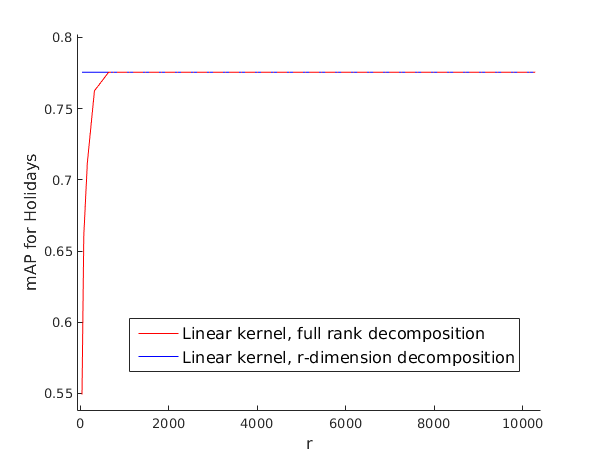
\includegraphics[width=\textwidth]{linear_decomposition_nolog.png}
%\end{subfigure}
%\begin{subfigure}[b]{0.48\textwidth}
%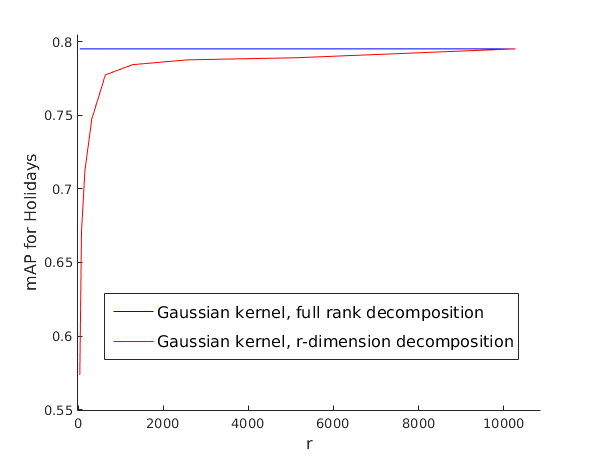
\includegraphics[width=\textwidth]{rbf_decomposition_nolog.png}
%\end{subfigure}
%\caption{Comparison between full rank and low rank. In blue, mAP results for full rank SLEM. %In red, mAP results for low rank decomposition of SLEM, varying the rank $r'$.
%At the left, linear SLEM results;at the right, Gaussian SLEM results. In this experiment, $n=10281$.}
%\label{no.ker.vs.linear2}
%\end{figure}


ubsection{Spatial pyramid matching kernel}

\begin{table}[!h]
    \centering
    \begin{tabular}{|c|c|c|c|c|}
    \hline
    Dataset & \multicolumn{2}{|c|}{\textbf{Holidays}} & \multicolumn{2}{|c|}{\textbf{Oxford 5k}}\\
    \hline
        Method, feaures & RootSIFT & CNN & RootSIFT
        &CNN \\
    \hline
    \hline
        SP SLEM & 66.9 & 70.2 & 42.4 & 45 \\
    \hline
    \end{tabular}
    \caption{Results }
    \label{tab:spk}
\end{table}
All previous kernel functions take as input image representations in a fixed sized vectorial space. In this section, we propose using the spatial pyramid kernel \cite{GrauDa05}, that takes as input a set of local descriptors and its coordinates in the image.

We revisit the spatial pyramid scheme presented in \cite{spk} using the generalized intersection function of histograms. 

Let $X$, $Y$ be the sets of local descriptors of a pair of images. 
These local descriptors can be associated to one of $M$ codewords $\{c_1,c_2,...,c_M\}$, so that $X=\bigcup_{1\leq m \leq M}X_m$ and $Y=\bigcup_{1\leq m \leq M}Y_m$, so that $X_m$, $Y_m$ are the set of descriptors associated to $c_m$. 
For level $l$ in $\{0,1,..., L\}$, we divide the images in grids $2^l\times 2^l$ and we call $H^{(l,m)}_X$, $H^{(l,m)}_Y$ the $4^l$-dimensional histograms of the occurrences of the of the visual word $c_m$ in each bin of the grid. 
The kernel $K_{sp}(X,Y)$ is given by sum over all codewords of the intersection histogram of $H^{(l,m)}_X$ and $H^{(l,m)}_Y$, $l=0,...,L$,  weighted proportionally to the number of bins in each level.

We test this kernel for RootSIFT extracted in multiscales, as used in \cite{spk}, and learn the codewords with K-means. Inspired by the results of \cite{SPPCNN}, we also test it for activations of the last convolutional layer of the network of \cite{SimonZisser15}. Each neuron of the last layer correspont to a codeword. The results are presented in Table \ref{tab:spk}.
%The spatial pyramid kernel is given by
%\begin{align}
%    K_{sp}(X,Y) &= \sum_{m=1}^M \kappa^L(X_m, Y_m), \ where \\
%    \kappa^L(X_m,Y_m) &= 2^{-L}I^{l}(X_m,Y_m) +\sum_{l=1}^L 2^{-L+l-1}I^{l}(X_m,Y_m) \label{kappa}\\
%    I^{l}(X_m,Y_m) = \sum_{i=1}^{4^l}\min()
%\end{align}

